% Agentic Coding Assistants: A Comparative Study of GitHub Copilot, Cursor, Claude Code and Codex
% IEEE conference format, 6-page target. Build: see paper/README.md (latexmk -pdf main.tex).
% Tables in tables/ and references.bib are generated by build_tables.py from evidence/*.json.
\documentclass[conference]{IEEEtran}
\usepackage[T1]{fontenc}
\usepackage{cite}
\usepackage{booktabs}
\usepackage{xcolor}
\usepackage{array}
\usepackage{url}
\usepackage[hidelinks]{hyperref}
\providecommand{\pilotstatus}{pending}
\usepackage{graphicx}
% Generated by paper/build_tables.py from analysis/swebench/output/summary.json
\newcommand{\swevSubs}{122}
\newcommand{\swevFirst}{32.6}
\newcommand{\swevBest}{79.2}
\newcommand{\swevBestName}{Sonar Foundation Agent + Claude 4.5 Opus}
\newcommand{\swevMedian}{57.0}
\newcommand{\swevNever}{29}
\newcommand{\swevEasy}{95}
\newcommand{\swevRepoLo}{68.4\% (sphinx-doc/sphinx)}
\newcommand{\swevRepoHi}{90.9\% (scikit-learn/scikit-learn)}
\newcommand{\swevSpreadModel}{claude-3-5-sonnet-20241022}
\newcommand{\swevSpreadMin}{33.6}
\newcommand{\swevSpreadMax}{63.4}
\newcommand{\swevSpreadAgents}{16}
\newcommand{\swevEntries}{182}


\begin{document}

\title{Agentic Coding Assistants: A Comparative Study of GitHub Copilot, Cursor, Claude Code and Codex}

% TODO: replace the placeholders with the author team before submission.
\author{\IEEEauthorblockN{Author Names}
\IEEEauthorblockA{Department, Institution, City, Country\\
email@example.org}}

\maketitle

\begin{abstract}
AI coding assistants have moved from inline completion to agents that plan, edit many files, run tests and
open pull requests (PRs) on their own. Evidence about them is scattered across benchmark leaderboards,
mining studies of agent-authored PRs and productivity experiments, and the four most visible products are
rarely compared on the same footing. We compare GitHub Copilot, Cursor, Claude Code and OpenAI Codex along
four dimensions---autonomy, context handling, tooling and deployment---and synthesise published evidence on
benchmark performance, PR acceptance, task-type dependence, post-merge quality, productivity and security.
Three findings stand out. First, reported acceptance rankings are not stable: across three studies of the
same AIDev data, Codex and Claude Code swap first place, while Copilot ranks last in all three. Second, task
type matters as much as the agent: acceptance differs by up to 29 percentage points between task categories,
and maintenance work is accepted far more often than features, fixes and performance changes. Third, merge
is a weak proxy for quality, since merged agent PRs still carry code smells and review is often absent. A re-analysis of \swevSubs{} SWE-bench Verified leaderboard submissions shows that the scaffold
around a model moves its score by up to 30 points, that results vary by repository, and that none of the
four products has been evaluated on the benchmark as shipped. We release a verified evidence registry,
the re-analysis, an AIDev re-analysis script and a product-level SWE-bench Verified pilot protocol.
\end{abstract}

\begin{IEEEkeywords}
AI coding assistants, software engineering agents, SWE-bench, pull requests, empirical software engineering
\end{IEEEkeywords}

% =====================================================================================================
\section{Introduction}

Code assistants began as autocomplete: a model proposes the next lines and the developer accepts or
rejects them. Current tools also act as \emph{agents}. They read a repository, plan a change, edit files,
execute commands and tests, and, in their asynchronous modes, return a branch or open a PR for review. In
the AIDev dataset alone, five agents authored 932,791 PRs in 116,211 GitHub repositories before August
2025~\cite{li2026aidev}.

Practitioners choosing among these tools face three gaps. Benchmarks such as SWE-bench~\cite{jimenez2024swebench}
score \emph{models inside research scaffolds}, not the products developers install. Mining studies of
agentic PRs~\cite{li2025teammates,rahman2026,mazloomzadeh2026,pinna2026} measure real outcomes but differ
in filters, task taxonomies and statistics, so their rankings are hard to compare. Productivity and
security studies~\cite{peng2023copilot,cui2025effects,perry2023insecure} mostly predate agentic modes.

The closest prior work, Pinna et al.~\cite{pinna2026}, stratifies 7,156 AIDev PRs from five agents by task
type. It reports a 29-point acceptance gap between task types and no single agent that leads every
category. We build on it in three ways. We add a product-level feature comparison that explains
\emph{why} the agents differ in what they are used for. We set PR acceptance against benchmark,
post-merge quality, productivity and security evidence rather than treating it alone. We also make the
synthesis checkable: every figure is traced to its source in a public registry, and inconsistencies found
while checking are reported.

\textbf{Contributions.}
(1) A structured comparison of Copilot, Cursor, Claude Code and Codex on autonomy, context handling,
tooling and deployment (Section~\ref{sec:compare}).
(2) A cross-study synthesis of evaluation evidence showing where conclusions agree and where they depend on
method (Section~\ref{sec:evidence}).
(3) A risk analysis covering security, technical debt, review burden and the benchmark-to-practice gap
(Section~\ref{sec:risks}).
(4) A re-analysis of per-instance results from \swevSubs{} SWE-bench Verified submissions
(Section~\ref{sec:swev}).
(5) Open instruments: a verified evidence registry, an AIDev re-analysis script and a SWE-bench Verified
pilot protocol for the four products.

% =====================================================================================================
\section{Background}

\subsection{From Codex to agents}
OpenAI's 2021 Codex \emph{model} powered the first GitHub Copilot, which offered single-file inline
completion. Chat interfaces followed, then IDE \emph{agent modes} that edit several files and run
commands, then asynchronous agents that work in a cloud sandbox and return PRs. The product now called
OpenAI Codex is such an agent, distinct from the 2021 model; we use ``Codex'' only for the product.

\subsection{Agent architecture}
Research agents make the common architecture explicit. SWE-agent showed that a purpose-built
agent--computer interface for searching, viewing and editing files raises issue resolution well above
non-interactive prompting~\cite{yang2024sweagent}. AutoCodeRover combines program-structure-aware code
search with spectrum-based fault localisation~\cite{zhang2024autocoderover}. OpenHands provides an open
platform in which agents write code, use a shell and browse, evaluated on 15 benchmarks~\cite{wang2025openhands}.
All share four capabilities: \emph{planning} a change, \emph{tool use} (shell, editor, tests, external
services), \emph{repository navigation} to find relevant code, and \emph{execution} to check the result.

\subsection{Interaction modes}
We distinguish four modes, which define the autonomy scale in Table~\ref{tab:features}: inline
suggestion (L1), conversational editing (L2), supervised local agents that act in the developer's
environment with approvals (L3), and asynchronous PR-submitting agents that work remotely and hand back a
diff or PR (L4).

% =====================================================================================================
\section{Methodology}

\subsection{Dimensions and selection}
We compare the assistants on \emph{autonomy} (highest mode offered), \emph{context handling} (how
repository knowledge and project instructions reach the agent), \emph{tooling} (extension points such as
the Model Context Protocol, hooks and custom agents) and \emph{deployment} (where the agent executes and
what it returns). The four products were chosen because each offers an agentic mode, each is covered in
the AIDev dataset~\cite{li2026aidev}, and together they span IDE-first (Copilot, Cursor) and agent-first
(Claude Code, Codex) designs. Feature data come from vendor documentation checked on 9~November~2026.

\subsection{Data sources}
We use two kinds of secondary evidence. \emph{Public benchmarks}: SWE-bench~\cite{jimenez2024swebench},
its human-validated Verified subset~\cite{openai2024verified}, and derivatives that address validity
(SWE-Bench+~\cite{aleithan2024swebenchplus}), modality (SWE-bench Multimodal~\cite{yang2025multimodal})
and scale (SWE-smith~\cite{yang2025swesmith}, SWE-Bench++~\cite{wang2025swebenchpp}). \emph{Agentic PR
datasets}: AIDev~\cite{li2026aidev} and studies built on it~\cite{li2025teammates,rahman2026,mazloomzadeh2026,pinna2026,cynthia2026postmerge,cynthia2026core}.
Productivity and security evidence comes from controlled and field experiments~\cite{peng2023copilot,cui2025effects,perry2023insecure,pearce2025asleep}.
Each figure was checked against the source text and recorded with its conditions in the evidence registry;
where a source has several versions, we name the one quoted.

\subsection{Instruments}
To move from secondary to primary evidence, we use three instruments. A SWE-bench Verified
re-analysis reads the per-instance results of every leaderboard submission from the official
experiments repository~\cite{swebench2026experiments}; we keep the \swevSubs{} submissions evaluated on
all 500 instances. It computes the state of the art over time, each instance's empirical difficulty (the
share of submissions resolving it), resolve rates by repository and issue year, and the spread of
scores for one model under different scaffolds. An AIDev re-analysis computes
merged/closed acceptance by agent and task type with Wilson intervals and Holm-corrected chi-square tests,
following~\cite{pinna2026}. A SWE-bench Verified pilot draws 12 instances, four from each tertile of empirical
difficulty and spread across repositories (seed 2026), has an operator work each one with each product under a fixed prompt and time limit in our
platform, which records time, follow-up prompts and interventions, and scores the patches with the
official harness. The platform also keeps an 18-task synthetic suite for task categories SWE-bench
does not isolate (security remediation, test writing, refactoring).
% swebench_pilot/results.csv not found: pilot not yet run.
\renewcommand{\pilotstatus}{pending, and no pilot results are reported here}%
At the time of writing the pilot is \pilotstatus.

\subsection{Limitations of cross-tool comparison}
Products change monthly and use different underlying models. AIDev attributes PRs only where agents leave
traces; Codex, for instance, adds no authorship metadata~\cite{li2025teammates}, and Claude Code's
co-author line can be disabled. Usage volumes are very unequal (e.g., 21,799 Codex versus 459 Claude Code
PRs in~\cite{rahman2026}), and users self-select which tasks to delegate. Benchmark scores attach to
model-plus-scaffold combinations, not to products.

% =====================================================================================================
\section{Comparative Analysis}\label{sec:compare}

% Generated from evidence/assistant_features.json (checked 2026-11-09). Do not edit by hand.
\begin{table*}[t]
\caption{Feature comparison of the four assistants (vendor documentation, checked 2026-11-09)}
\label{tab:features}
\centering\scriptsize
\begin{tabular}{@{}p{0.08\textwidth}p{0.17\textwidth}p{0.05\textwidth}p{0.19\textwidth}p{0.15\textwidth}p{0.26\textwidth}@{}}
\toprule
Assistant & Interaction modes & Auton. & Context handling & Tooling & Execution and deployment\\
\midrule
GitHub Copilot & Inline completion; Chat; IDE agent mode; Cloud agent assigned from issues, chat or agent panel & L1--L4 & Repository-scoped; GitHub MCP server gives issue and PR history; custom instructions at personal, repository and organisation level & MCP servers, custom agents, agent skills, hooks & Cloud agent runs in a temporary cloud development environment, edits, runs tests and linters. Creates a branch and opens one PR per task; 59-minute session cap; rulesets can block it\\
Cursor & AI-native editor with Tab completion; In-editor Agent; Cloud Agents launched from editor, web, mobile, Slack, GitHub or Linear & L1--L4 & Indexed workspace in the editor; cloud agents get the repo, dependencies and configured secrets & Editor tools, terminal, MCP; per-environment secrets and network policies & Cloud Agents run in a separate sandboxed VM per agent. Cloud agents can open a PR with videos, screenshots and logs attached\\
Claude Code & Terminal CLI agent; VS Code and JetBrains extensions; Desktop app; Web and mobile cloud sessions; Slack and CI (GitHub Actions, GitLab CI/CD) & L3--L4 & Reads the codebase on demand; CLAUDE.md (or AGENTS.md) project instructions; auto memory & MCP, skills, hooks, subagents, Agent SDK & Runs commands locally under a permission system, or in cloud sessions. Stages, commits, creates branches and opens PRs; Slack mention can return a PR\\
OpenAI Codex & Cloud tasks (web/ChatGPT); Codex CLI; IDE extension & L3--L4 & Checks out the repo at a branch/commit; AGENTS.md tells the agent lint and test commands & Terminal in a container; setup and maintenance scripts; MCP in the CLI & Cloud container from the 'universal' image; internet off by default during the agent phase (setup scripts may use it). Returns an answer and a diff; the user opens a PR from it\\
\bottomrule
\multicolumn{6}{@{}p{0.95\textwidth}@{}}{\emph{Autonomy scale.} L1: Suggestion: inline completion the developer accepts or rejects; L2: Conversational: chat proposes edits; developer applies them; L3: Supervised local agent: plans, edits files and runs commands in the developer's environment, with approvals; L4: Asynchronous delegated agent: works in a remote sandbox and returns a branch, diff or pull request for review}\\
\end{tabular}
\end{table*}


\textbf{GitHub Copilot} spans all four modes. Its cloud agent is assigned work from issues, chat or an
agent panel, runs in a temporary cloud environment, and opens one PR per task on one branch, with a
59-minute session limit and only for GitHub-hosted repositories. Repository context arrives through the
GitHub MCP server and layered custom instructions.

\textbf{Cursor} is an AI-native editor. Tab completion and an in-editor agent cover L1--L3. Cloud agents
(L4) each run in a sandboxed virtual machine and can be launched from the editor, web, mobile, Slack, GitHub
or Linear. They can attach screenshots, videos and logs to the PRs they open.

\textbf{Claude Code} is agent-first, with no inline completion. The same engine runs in a terminal, IDE
extensions, a desktop app, the web and CI. It edits files and runs commands under a permission system,
and it commits and opens PRs itself. Project knowledge comes from \texttt{CLAUDE.md} files and auto
memory; extension points are MCP, skills, hooks and subagents.

\textbf{OpenAI Codex} runs tasks in cloud containers built from a common image after a setup script.
Internet access is off by default during the agent phase. The agent returns an answer and a diff, from
which the user opens a PR. \texttt{AGENTS.md} supplies lint and test commands; a CLI and an IDE extension
cover local use.

Two design differences recur in the evidence below. The IDE-first tools expose low-autonomy modes alongside
agents, so their PR streams include work started interactively. The agent-first tools make the agent the
default unit of work, so delegated tasks may be larger. The feature table cannot say which design produces
better outcomes; it frames what the outcome data mean.

% =====================================================================================================
\section{Evaluation Evidence}\label{sec:evidence}

\subsection{SWE-bench and derivatives}
% Generated from evidence/evidence.json. Do not edit by hand.
\begin{table}[t]
\caption{SWE-bench family: reported results and validity findings}
\label{tab:benchmarks}
\centering\scriptsize
\begin{tabular}{@{}p{0.27\columnwidth}p{0.42\columnwidth}r@{\ }l@{}}
\toprule
System / set & Metric & \multicolumn{2}{l}{Value}\\
\midrule
Claude 2 (RAG baseline) & SWE-bench resolve rate & 1.96\% & \cite{jimenez2024swebench}\\
SWE-bench Verified & Instances & 500 & \cite{openai2024verified}\\
GPT-4o (best open scaffold) & Resolve rate, Verified vs original & 33.2\% & \cite{openai2024verified}\\
SWE-agent & SWE-bench pass@1 & 12.5\% & \cite{yang2024sweagent}\\
AutoCodeRover & SWE-bench Lite resolve rate & 19\% & \cite{zhang2024autocoderover}\\
SWE-agent & SWE-bench Multimodal resolve rate & 12\% & \cite{yang2025multimodal}\\
SWE-agent-LM-32B & SWE-bench Verified pass@1 & 40.2\% & \cite{yang2025swesmith}\\
claude-sonnet-4.5 & SWE-Bench++ pass@10 & 36.2\% & \cite{wang2025swebenchpp}\\
Best reported system (Claude Opus 4.7) & SWE-bench Verified resolve rate (survey trajectory) & 78.4\% & \cite{bhati2026}\\
SWE-Agent + GPT-4 passing patches & Solution leakage in issue text & 32.67\% & \cite{aleithan2024swebenchplus}\\
SWE-Agent + GPT-4 on Verified & Resolve rate before vs after filtering & 10\% & \cite{aleithan2024swebenchplus}\\
AutoCodeRover + GPT-4o & SWE-Bench+ resolve rate & 3.83\% & \cite{aleithan2024swebenchplus}\\
8 agents on Verified & Resolution when a task had more than 20 execution errors & 22.6\% & \cite{chen2026beyond}\\
\bottomrule
\end{tabular}
\end{table}

SWE-bench poses 2,294 real issues from 12 Python repositories; the best baseline in the original paper
resolved 1.96\%~\cite{jimenez2024swebench}. SWE-bench Verified keeps 500 instances that developers judged
well specified and fairly tested; 68.3\% of annotated samples were removed~\cite{openai2024verified}.
Reported Verified scores have since risen to about 78\% for the best model-plus-scaffold
combination~\cite{bhati2026}. Derivatives show the limits of these numbers (Table~\ref{tab:benchmarks}).
In SWE-Bench+, 32.67\% of passing patches had the fix stated in the issue text and 31.08\% passed only
because tests were weak; on post-cutoff issues, a system reported at 18.83\% fell to
3.83\%~\cite{aleithan2024swebenchplus}. Moving to JavaScript with visual issues drops the best system to
12\%~\cite{yang2025multimodal}, and multilingual tasks from live PRs yield at most 36.2\%
pass@10~\cite{wang2025swebenchpp}.

\subsection{Re-analysis of Verified leaderboard submissions}\label{sec:swev}
% Generated by analysis/swebench/verified_analysis.py from SWE-bench/experiments @ 40f164d5b8
\begin{table}[t]
\caption{SWE-bench Verified leaderboard re-analysis (this study): 122 submissions on all 500 instances}
\label{tab:swev}
\centering\scriptsize
\begin{tabular}{@{}lr@{\hspace{1.2em}}lr@{}}
\toprule
\multicolumn{2}{@{}l}{Instances by share of submissions resolving them} & \multicolumn{2}{l@{}}{Top-10 mean rate by issue year} \\
\midrule
never solved & 29 & 2017 ($n$=16) & 90.6\%\\
under 10\% & 57 & 2018 ($n$=24) & 74.2\%\\
10-50\% & 113 & 2019 ($n$=98) & 81.6\%\\
50-90\% & 206 & 2020 ($n$=108) & 80.7\%\\
90\% or more & 95 & 2021 ($n$=86) & 69.5\%\\
& & 2022 ($n$=102) & 75.5\%\\
& & 2023 ($n$=58) & 75.9\%\\
\midrule
\multicolumn{4}{@{}l}{Top-10 mean rate by repository (largest five)}\\
\multicolumn{3}{@{}l}{django/django ($n$=231)} & 80.6\%\\
\multicolumn{3}{@{}l}{sympy/sympy ($n$=75)} & 74.3\%\\
\multicolumn{3}{@{}l}{sphinx-doc/sphinx ($n$=44)} & 68.4\%\\
\multicolumn{3}{@{}l}{matplotlib/matplotlib ($n$=34)} & 73.5\%\\
\multicolumn{3}{@{}l}{scikit-learn/scikit-learn ($n$=32)} & 90.9\%\\
\bottomrule
\end{tabular}
\end{table}

\begin{figure}[t]
\centering
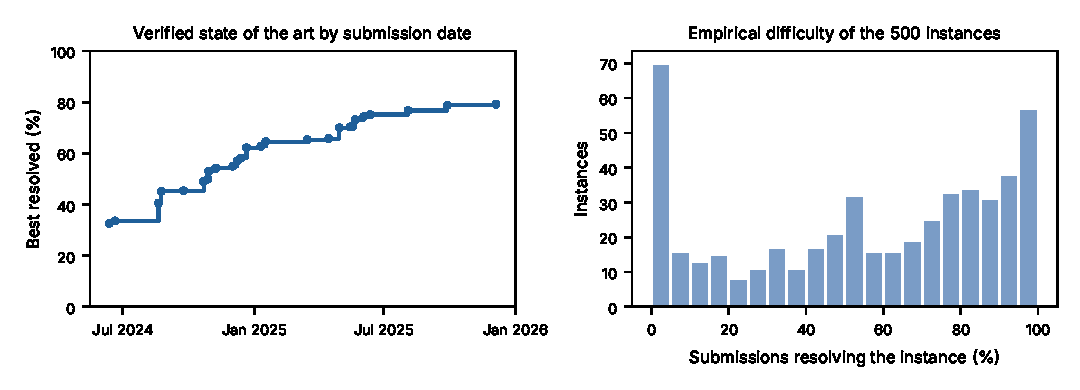
\includegraphics[width=\columnwidth]{figures/swebench_verified.pdf}
\caption{SWE-bench Verified, this study's re-analysis of \swevSubs{} submissions. Left: best resolve
rate by submission date. Right: share of submissions that resolve each instance.}
\label{fig:swev}
\end{figure}
Across the \swevSubs{} complete submissions (June 2024 to September 2026), the best resolve rate rose from
\swevFirst\% to \swevBest\% and the median submission resolves \swevMedian\% (Fig.~\ref{fig:swev}).
Difficulty is very uneven: \swevNever{} instances were never resolved by any submission, while
\swevEasy{} are resolved by 90\% or more (Table~\ref{tab:swev}). Repository matters even at the top:
the ten best submissions average \swevRepoLo{} to \swevRepoHi{} across the five largest repositories.
The scaffold matters as much as the model. The same model, \texttt{\swevSpreadModel}, scores between
\swevSpreadMin\% and \swevSpreadMax\% under \swevSpreadAgents{} different agents. Resolve rates show no
steady decline with issue year, so this coarse test finds no simple contamination signal. Finally, we
searched all \swevEntries{} Verified entries and the four other SWE-bench leaderboards~\cite{swebench2026leaderboard}.
None is GitHub Copilot, Cursor, Claude Code or the Codex product as shipped. The only Codex-branded
entries are OpenAI models run in the generic mini-SWE-agent scaffold (GPT~5.2 Codex 72.8\%, GPT~5.1
Codex 66.0\%). Benchmark numbers quoted for these products are model-level numbers, which is why we
designed the product-level pilot.

\subsection{PR acceptance and merge rates}
% Generated from evidence/evidence.json. Do not edit by hand.
\begin{table}[t]
\caption{Reported PR acceptance (\%) of the four assistants in three studies of AIDev data. Rank in parentheses.}
\label{tab:acceptance}
\centering\scriptsize
\begin{tabular}{@{}p{0.36\columnwidth}rrrr@{}}
\toprule
Study & Codex & Claude C. & Cursor & Copilot\\
\midrule
Li et al.~\cite{li2025teammates}, AIDev-pop & 65.3 (1) & 52.5 (2) & 51.4 (3) & 38.2 (4)\\
Rahman et al.~\cite{rahman2026}, mean over types & 83 (1) & 66 (3) & 67 (2) & 45 (4)\\
Mazloomzadeh et al.~\cite{mazloomzadeh2026}, GLMM & 73.5 (2) & 84.3 (1) & 63.9 (3) & 59.6 (4)\\
\bottomrule
\multicolumn{5}{@{}p{0.95\columnwidth}@{}}{Human PRs: 76.8\% in AIDev-pop~\cite{li2025teammates}; 84--86\% per quarter in~\cite{mazloomzadeh2026}.}\\
\end{tabular}
\end{table}

Table~\ref{tab:acceptance} sets the three studies that report all four assistants side by side. Copilot
ranks last in every study, while the order of Codex and Claude Code depends on the method. With raw merge
rates in high-star repositories, Codex leads~\cite{li2025teammates}; averaged over task types, Codex leads
again~\cite{rahman2026}; with a mixed model controlling for repository in Python projects, Claude Code
leads and its difference from Codex is not significant~\cite{mazloomzadeh2026}. All agents trail human PRs
(76.8\% in~\cite{li2025teammates}). Developer role matters little to acceptance: core and peripheral
developers accept 72.8\% and 72.3\% of agentic PRs~\cite{cynthia2026core}.

\subsection{Task-type dependence}
Pinna et al.\ find a 29-point gap between the most and least accepted task types (chore 84.0\%, performance
55.4\%)~\cite{pinna2026}; their later revision highlights documentation versus features (82.1\% vs.\
66.1\%). Every study agrees on direction: documentation, CI, build and dependency work is accepted more
often than features, fixes and performance changes~\cite{rahman2026,mazloomzadeh2026,li2025teammates}. On
documentation, Codex (88.6\%) and Claude Code (85.7\%) exceed human PRs (76.5\%), while agents trail humans
by 15--40 points on features, fixes and performance~\cite{li2025teammates}. Agents also differ in what they
are given: Claude Code's AIDev-pop PRs are 49.5\% features, while Copilot's are 42.2\% fixes. Comparisons
that ignore task mix therefore conflate tool quality with delegation habits.

\subsection{Post-merge quality and regressions}
Merge is not the end of the story. In 1,210 merged agent bug-fix PRs, SonarQube found 1,190 new issues:
89\% code smells, 48 bugs and 83 security hotspots. Differences between agents vanished once issue counts
were normalised by churn~\cite{cynthia2026postmerge}. Compared with human PRs, merged agentic PRs differ
little in size or time to merge~\cite{mazloomzadeh2026}. Regressions are a separate risk that resolution
rates hide: giving an agent a static code-to-test impact map cut test-level regressions from 6.08\% to
1.82\% on SWE-bench Verified, while TDD-style prompting alone raised them to 9.94\%~\cite{alonso2026tdad}.
Process data tell a similar story. Across eight agents, tasks with more than 20 execution errors were
resolved 22.6\% of the time, against 53.8\% with none~\cite{chen2026beyond}.

\subsection{Productivity evidence and its limits}
The strongest causal effects come from controlled tasks. Developers with Copilot built a JavaScript HTTP
server 55.8\% faster (95\% CI 21--89\%)~\cite{peng2023copilot}. Field experiments at Microsoft, Accenture and
a Fortune~100 firm with 4,867 developers found 26.08\% more completed tasks (SE 10.3\%), with larger gains
for less experienced developers~\cite{cui2025effects}. Effects shrink from controlled to field to
longitudinal settings~\cite{bhati2026}. All of this evidence concerns completion-era tools; no comparable
experiment exists yet for asynchronous agents.

% =====================================================================================================
\section{Risks}\label{sec:risks}

\textbf{Security.} In a user study, participants with an AI assistant wrote secure encryption code 21\% of
the time versus 43\% without one, and 36\% wrote SQL-injectable code versus 7\%. They also rated their code
as more secure~\cite{perry2023insecure}. Copilot suggestions have been shown to reproduce MITRE Top-25 CWE
weaknesses~\cite{pearce2025asleep}. Agent PRs add security hotspots even when no vulnerability is
confirmed~\cite{cynthia2026postmerge}.

\textbf{Technical debt.} Code smells dominate post-merge issues, with critical and major severities common;
the top rules are duplicated literals, cognitive complexity and unused parameters~\cite{cynthia2026postmerge}.
Because agents produce more PRs per developer, small per-PR debt compounds.

\textbf{Review burden.} 90.6\% of agentic PRs in one study had no recorded review comment, and 98.2\% of
Codex PRs~\cite{rahman2026}. 58.2\% of agent PRs had no review at all, against 75.3\% of human PRs in the
same repositories~\cite{li2025teammates}. Peripheral developers merged 19.1\% of their agentic PRs with no CI
checks, against 11.2\% for core developers~\cite{cynthia2026core}. Fast merges without review move
verification cost downstream rather than removing it.

\textbf{Benchmark-to-practice gap.} Leakage, weak tests and contamination inflate benchmark
scores~\cite{aleithan2024swebenchplus}. Scaffold choice alone moves one model's Verified score by about
30 points (Section~\ref{sec:swev}), so a product's own scaffold, defaults and limits cannot be inferred
from its model's leaderboard entry. Benchmark infrastructure itself had confirmed bugs~\cite{chen2026beyond}.
Benchmarks score models while practitioners buy products whose scaffolds, defaults and limits differ.
Secondary sources propagate errors: one survey describes Verified as 489 tasks rather than
500~\cite{bhati2026,openai2024verified}.

% =====================================================================================================
\section{Open Challenges}

\begin{itemize}
\item \emph{Product-level benchmarks.} Evaluate shipped assistants, with their own scaffolds and limits,
on contamination-resistant tasks, and report intervention counts alongside resolution.
\item \emph{Task-normalised outcome metrics.} Compare agents within task types and repositories, as the
mixed model in~\cite{mazloomzadeh2026} does, rather than by pooled merge rates.
\item \emph{Quality beyond merge.} Track regressions, reverts and maintenance cost of merged agent code
over time, not just static issues at merge.
\item \emph{Attribution.} Agent-authored work that leaves no trace biases every mining study; common
provenance metadata would help.
\item \emph{Review at scale.} Tooling that targets human review at risky agent changes, such as impact
analysis~\cite{alonso2026tdad}, instead of reviewing everything or nothing.
\item \emph{Agentic productivity.} Randomised field evidence for asynchronous agents does not yet exist.
\end{itemize}

% =====================================================================================================
\section{Conclusion}

Copilot, Cursor, Claude Code and Codex now all offer agents that submit PRs, but they reach that point from
different designs. The evidence agrees on several points: agents trail humans in acceptance, Copilot's PRs
are accepted least often, maintenance tasks fare best, and merged agent code still carries smells and
receives little review. It disagrees on which agent leads, and that ranking moves with the analysis method.
Benchmarks show fast model progress, from about a third to about four fifths of Verified issues in
eighteen months, but they measure neither products nor practice. Choosing an assistant
should therefore depend on the task mix, the review capacity of the team and the deployment constraints,
more than on a leaderboard position. Our registry, re-analysis script and pilot protocol are offered so
that these comparisons can be repeated as the tools change.

\bibliographystyle{IEEEtran}
\bibliography{references}

\end{document}
